\chapter{Semi-Shape-Preserved Clustering Representation}
This chapter introduces the proposed novel representation method that are temporarily named as \textbf{Semi-Shape-Preserved Clustering Representation (SSPCR)} and how it is designed according to the guideline of the project. \emph{Semi-Shape-Preserve} means that the generated feature vector contains the shape information of the original sequence while does not have the same visual appearance with it. \emph{Clustering} means that this method is designed for clustering tasks.

\section{Preliminaries}
\subsection{Reformulation of within-cluster-scatter}
\label{sec:reformulation}
The main objective of traditional clustering algorithms such as K-means is to minimize the total squared error between the data points and their representative center, this objective is termed as \textbf{within-cluster-scatter}. Let $x_i$ denotes a m-dimensional data vector, $i = 1,\cdots,n$, $X = [x_1, \cdots, x_n]$ denotes the $m \times n$ data matrix, $\Pi$ denotes the partition results, $k$ denotes the number of cluster, the objective function of K-means can be defined as below:
\begin{equation}
    \mathcal{L}_{clustering} = ss(\Pi) = \sum_{i=1}^k \sum_{s=1}^{s_i} \left\|x_s^{(i)} - m_i \right\|^2
    \label{eq:kmeans1}
\end{equation}
\begin{equation}
    m_i = \frac{\sum_{s=1}^{s_i} x_s^{(i)}}{s_i}
\end{equation}
$x_s^{(i)}$ represents the $s$th data vector in cluster $i$, and $m_i$ represents the mean vector of cluster $i$. According to \cite{zha2001spectral}, the minimization of $ss(\Pi)$ can be reformulated as a maximization of the trace of the Gram matrix $X^TX$ with spectral relaxation. Given the cluster indicator matrix $F \in \mathbb{R}^{n \times k}$, the Equation \ref{eq:kmeans1} can be re-written as:
\begin{equation}
    \mathcal{L}_{clustering} = ss(\Pi) = tr(X^TX) - tr(F^TX^TXF)
    \label{eq:kmeans2}
\end{equation}
$tr$ represents the function to compute the trace of a matrix. If the data matrix $X$ is fixed, the minimization of $ss(\Pi)$ can be relaxed to finding a $F$ with the constraints: (1) $F$ is an orthogonal matrix; (2) $F^TF = I$; (3) the trace of matrix $F^TX^TXF$ if maximized. The mathematical equation is defined as:
\begin{equation}
    \mathop{max} \limits_{F} \; tr(F^TX^TXF), s.t. F^TF = I
    \label{eq:kmeans3}
\end{equation}
This equation shows that the $F$ has a closed-form solution. Based on the Ky Fan theorem \cite{zha2001spectral}, there is an optimal $F$ that can be obtained by SVD decomposition of the data matrix $X$ and composing the first $k$ singular vectors. It's worth mentioning that this reformulation can lead to a global optimal solution, which may not be obtained with traditional approaches.

\subsection{Autoencoders}
As mentioned before, an autoencoder is a special neural network designed for dimension reduction/extension and feature extraction. A typical autoencoder consists of two components: (1) the encoder, which is in charge of transforming the original data vector into a new feature space; (2) the decoder, which takes the encoded vector and tries to reconstruct the original vector. Figure~\ref{fig:autoencoder1} shows the structure of traditional autoencoders. Some traditional autoencoders adpot a symmetric structure, where the encoder and decoder are mirror neural networks and share the same weights, but this is not required for all autoencoders. Generally, autoencoders generate two types of representations based on the dimensionality settings: (1) under-complete, when the dimension of the transformed vector is lower than that of the original vector; (2) over-complete, when the dimension of the transformed vector is higher than that of the original vector. First type can be used for data compression while the second type may capture intrinsic structures underlying data. The learning process of the representation is done by minimizing the reconstruction loss, given $x_i$ is the original vector and $\bar{x_i}$ is the transformed vector, the equation is defined as:
\begin{equation}
    \mathcal{L}_{reconstruction}(X) = \frac{1}{2|X|}\sum_{i=1}^{|X|} \left\|x_i - \bar{x_i} \right\|^2
    \label{eq:reconstruction}
\end{equation}
There are more sophisticated autoencoders with other constraints, but in general, they share the basic paradigm.
\begin{figure}[!htbp]
    \centering
    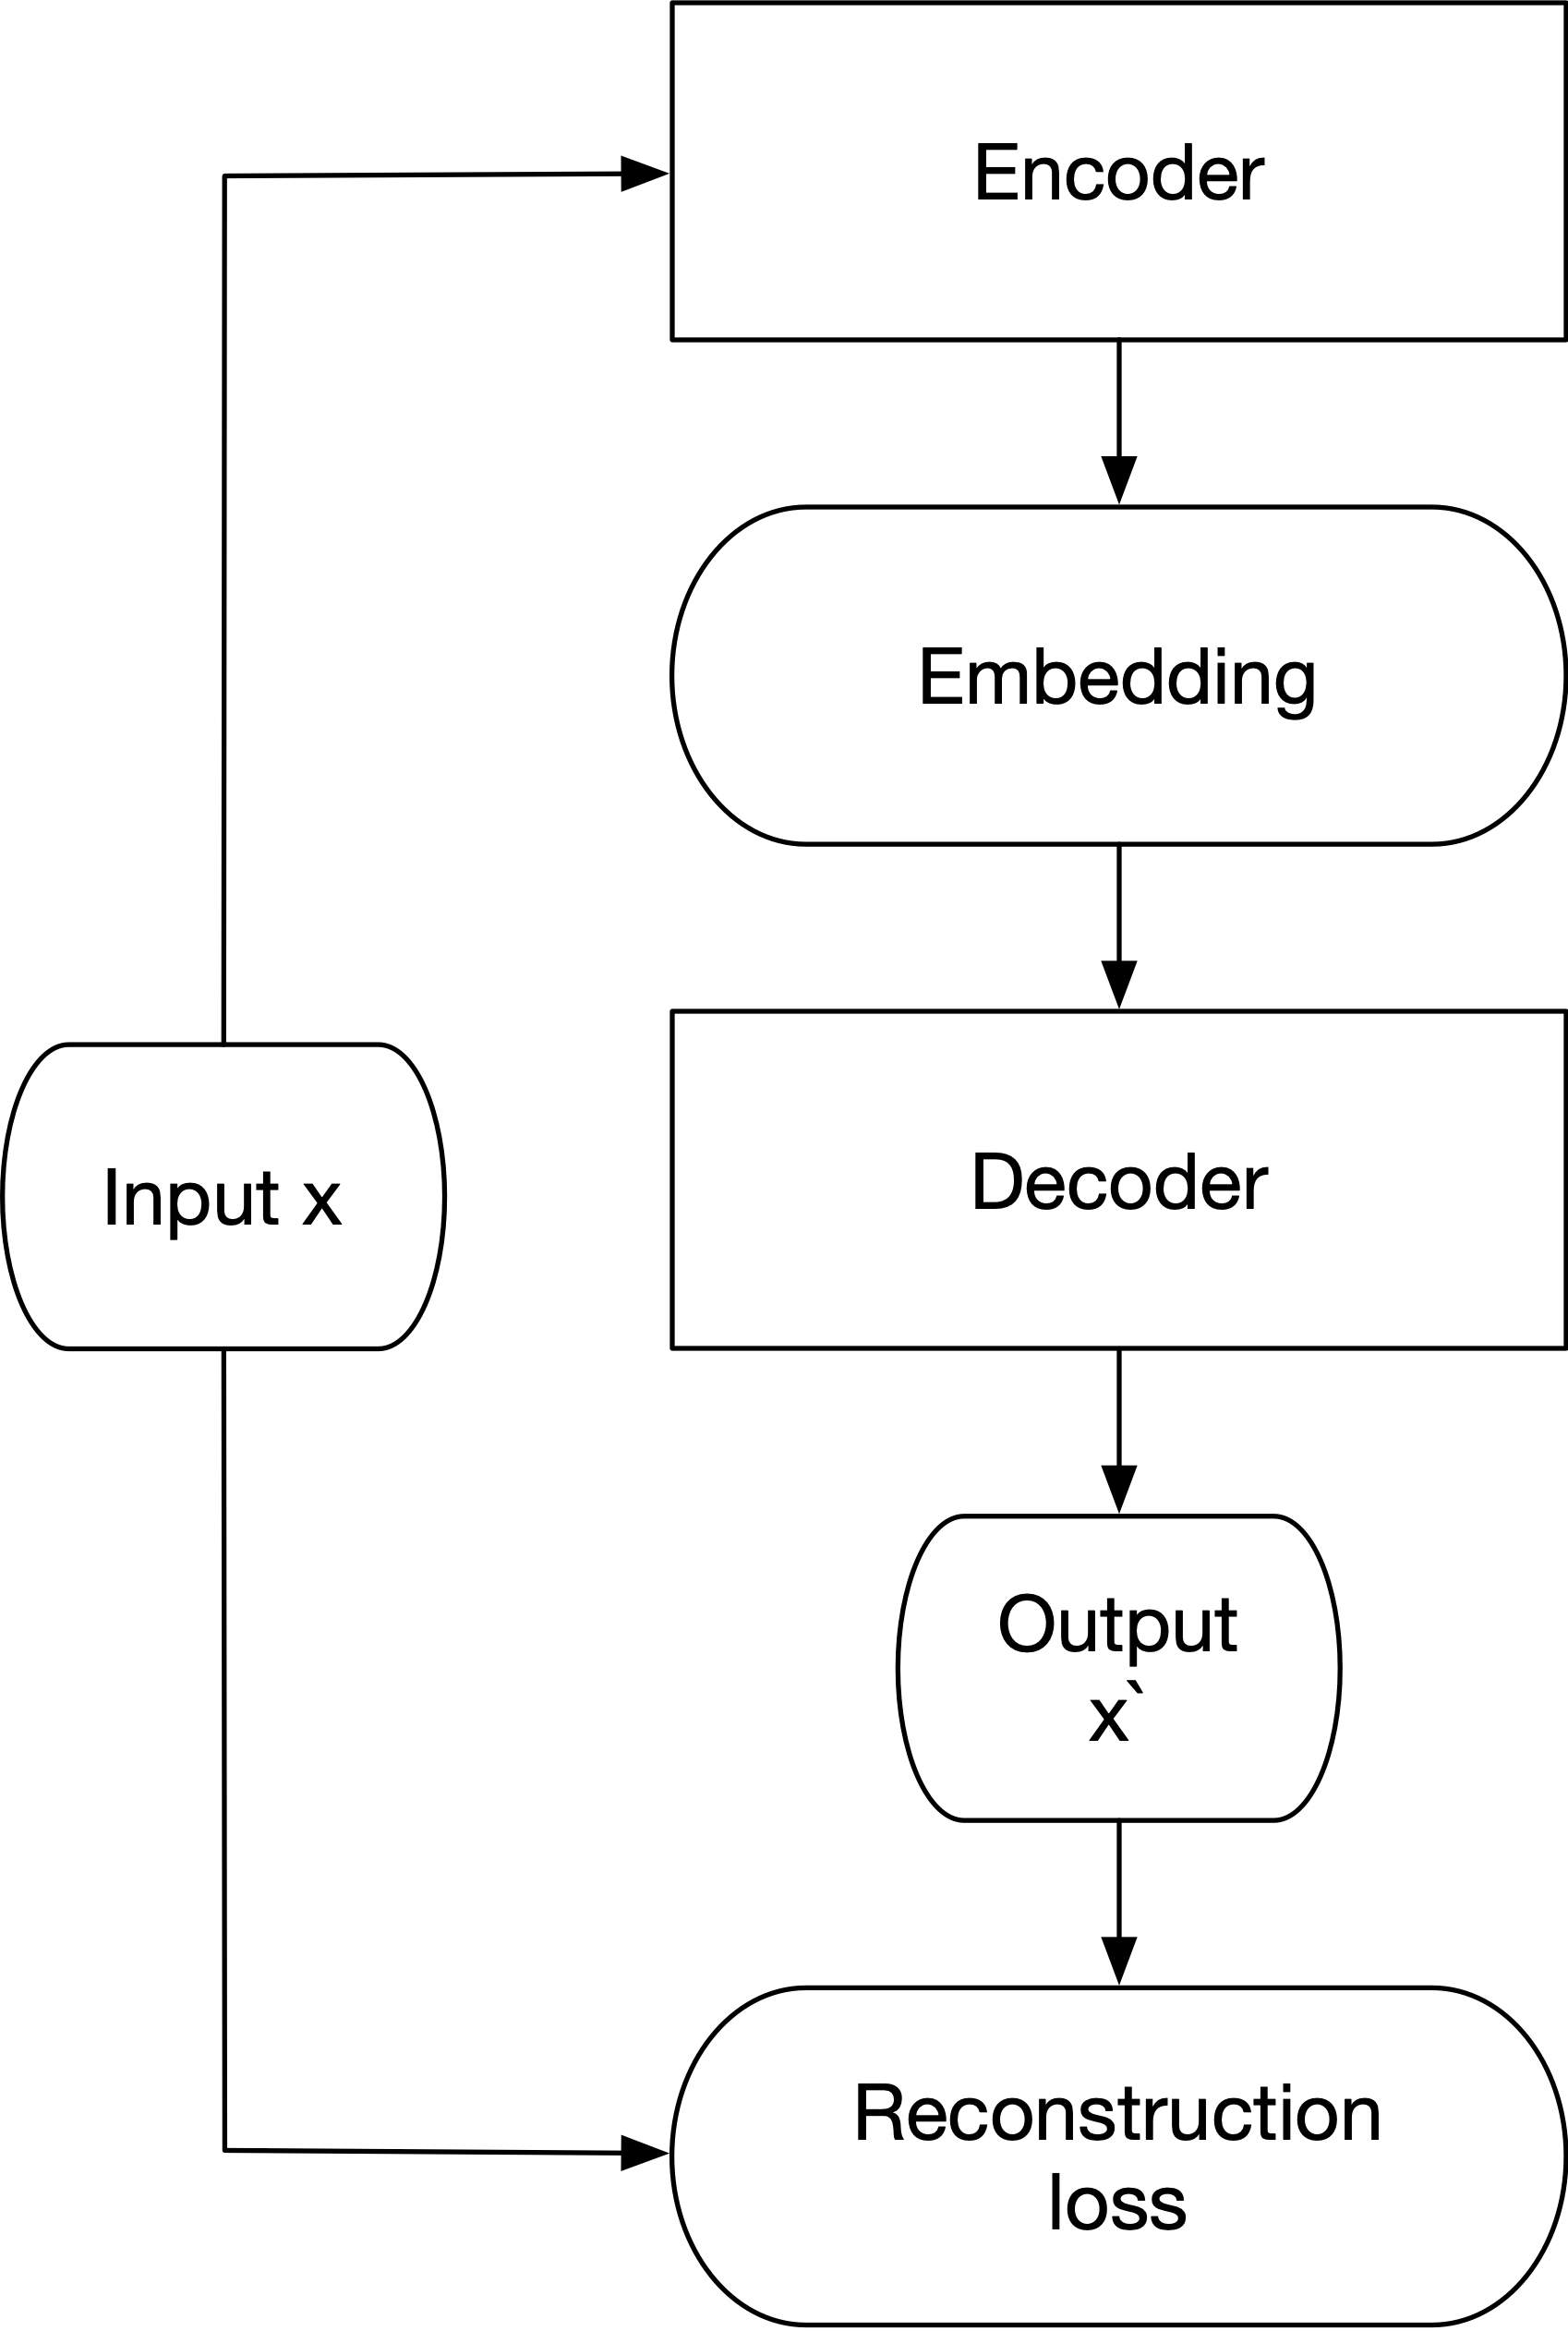
\includegraphics[width=0.3 \columnwidth]{autoencoder1.png}
    \caption{Structure of traditional autoencoders}
    \label{fig:autoencoder1}
\end{figure} 

\section{Algorithm Description}
In previous chapter, some shape-preserved and shape-changed representations are introduced, all those approaches are not designed for clustering tasks. As discussed before, shape-preserved representations are mainly static, and they indeed do not transform the new vectors into a new feature space. To the contrary, shape-changed representations have the ability to reveal the intrinsic properties of the original data, however, the transformed vectors could have quite different visual appearances with the raw sequences, leading the loss of shape information. Both of the two categories of representation approaches have their own advantages and disadvantages, and this motivates the proposition of SSPCR. The design guideline behind the proposed learning paradigm is to make the transformed vectors more distinguishable while preserving the most shape information.\\
\\When design SSPCR, the first question is how to force the representation to be encoded with the shape information. Since the dimension of the transformed vectors are usually different with that of the raw data vectors, directly approximating the original sequences are not feasible. Inspired by \cite{nanopoulos2001feature}, the general shape of a time-series sequence can be represented by a set of statistical features, this gives a hint that \textbf{if a transformed vector has the similar statistical features with that of its original vector, it can be said to preserve some of the shape information}. To make the learning paradigm appropriate for clustering tasks, the reformulation of within-cluster-scatter (see Section~\ref{sec:reformulation}) is introduced. This reformulation proves that given the data matrix, there is an optimal partition leading to the smallest within cluster scatter (i.e. the mostcompact clusters). More important, it shows how to get the best clustering result in terms of that objective function. This gives a hint that \textbf{if the transformed vectors have the smallest within cluster scatter computed by the reformulated equation, they can be said to be appropriate for clustering}. Having these two hints, the last question is how to get the representation. There may be a global optimal solution, but it could be hard to compute. Instead, \textbf{SSPCR treats finding the best representation as an optimization problem and adpots autoencoders with gradient descent to find a local optimal solution}.\\
\begin{figure}[!htbp]
    \centering
    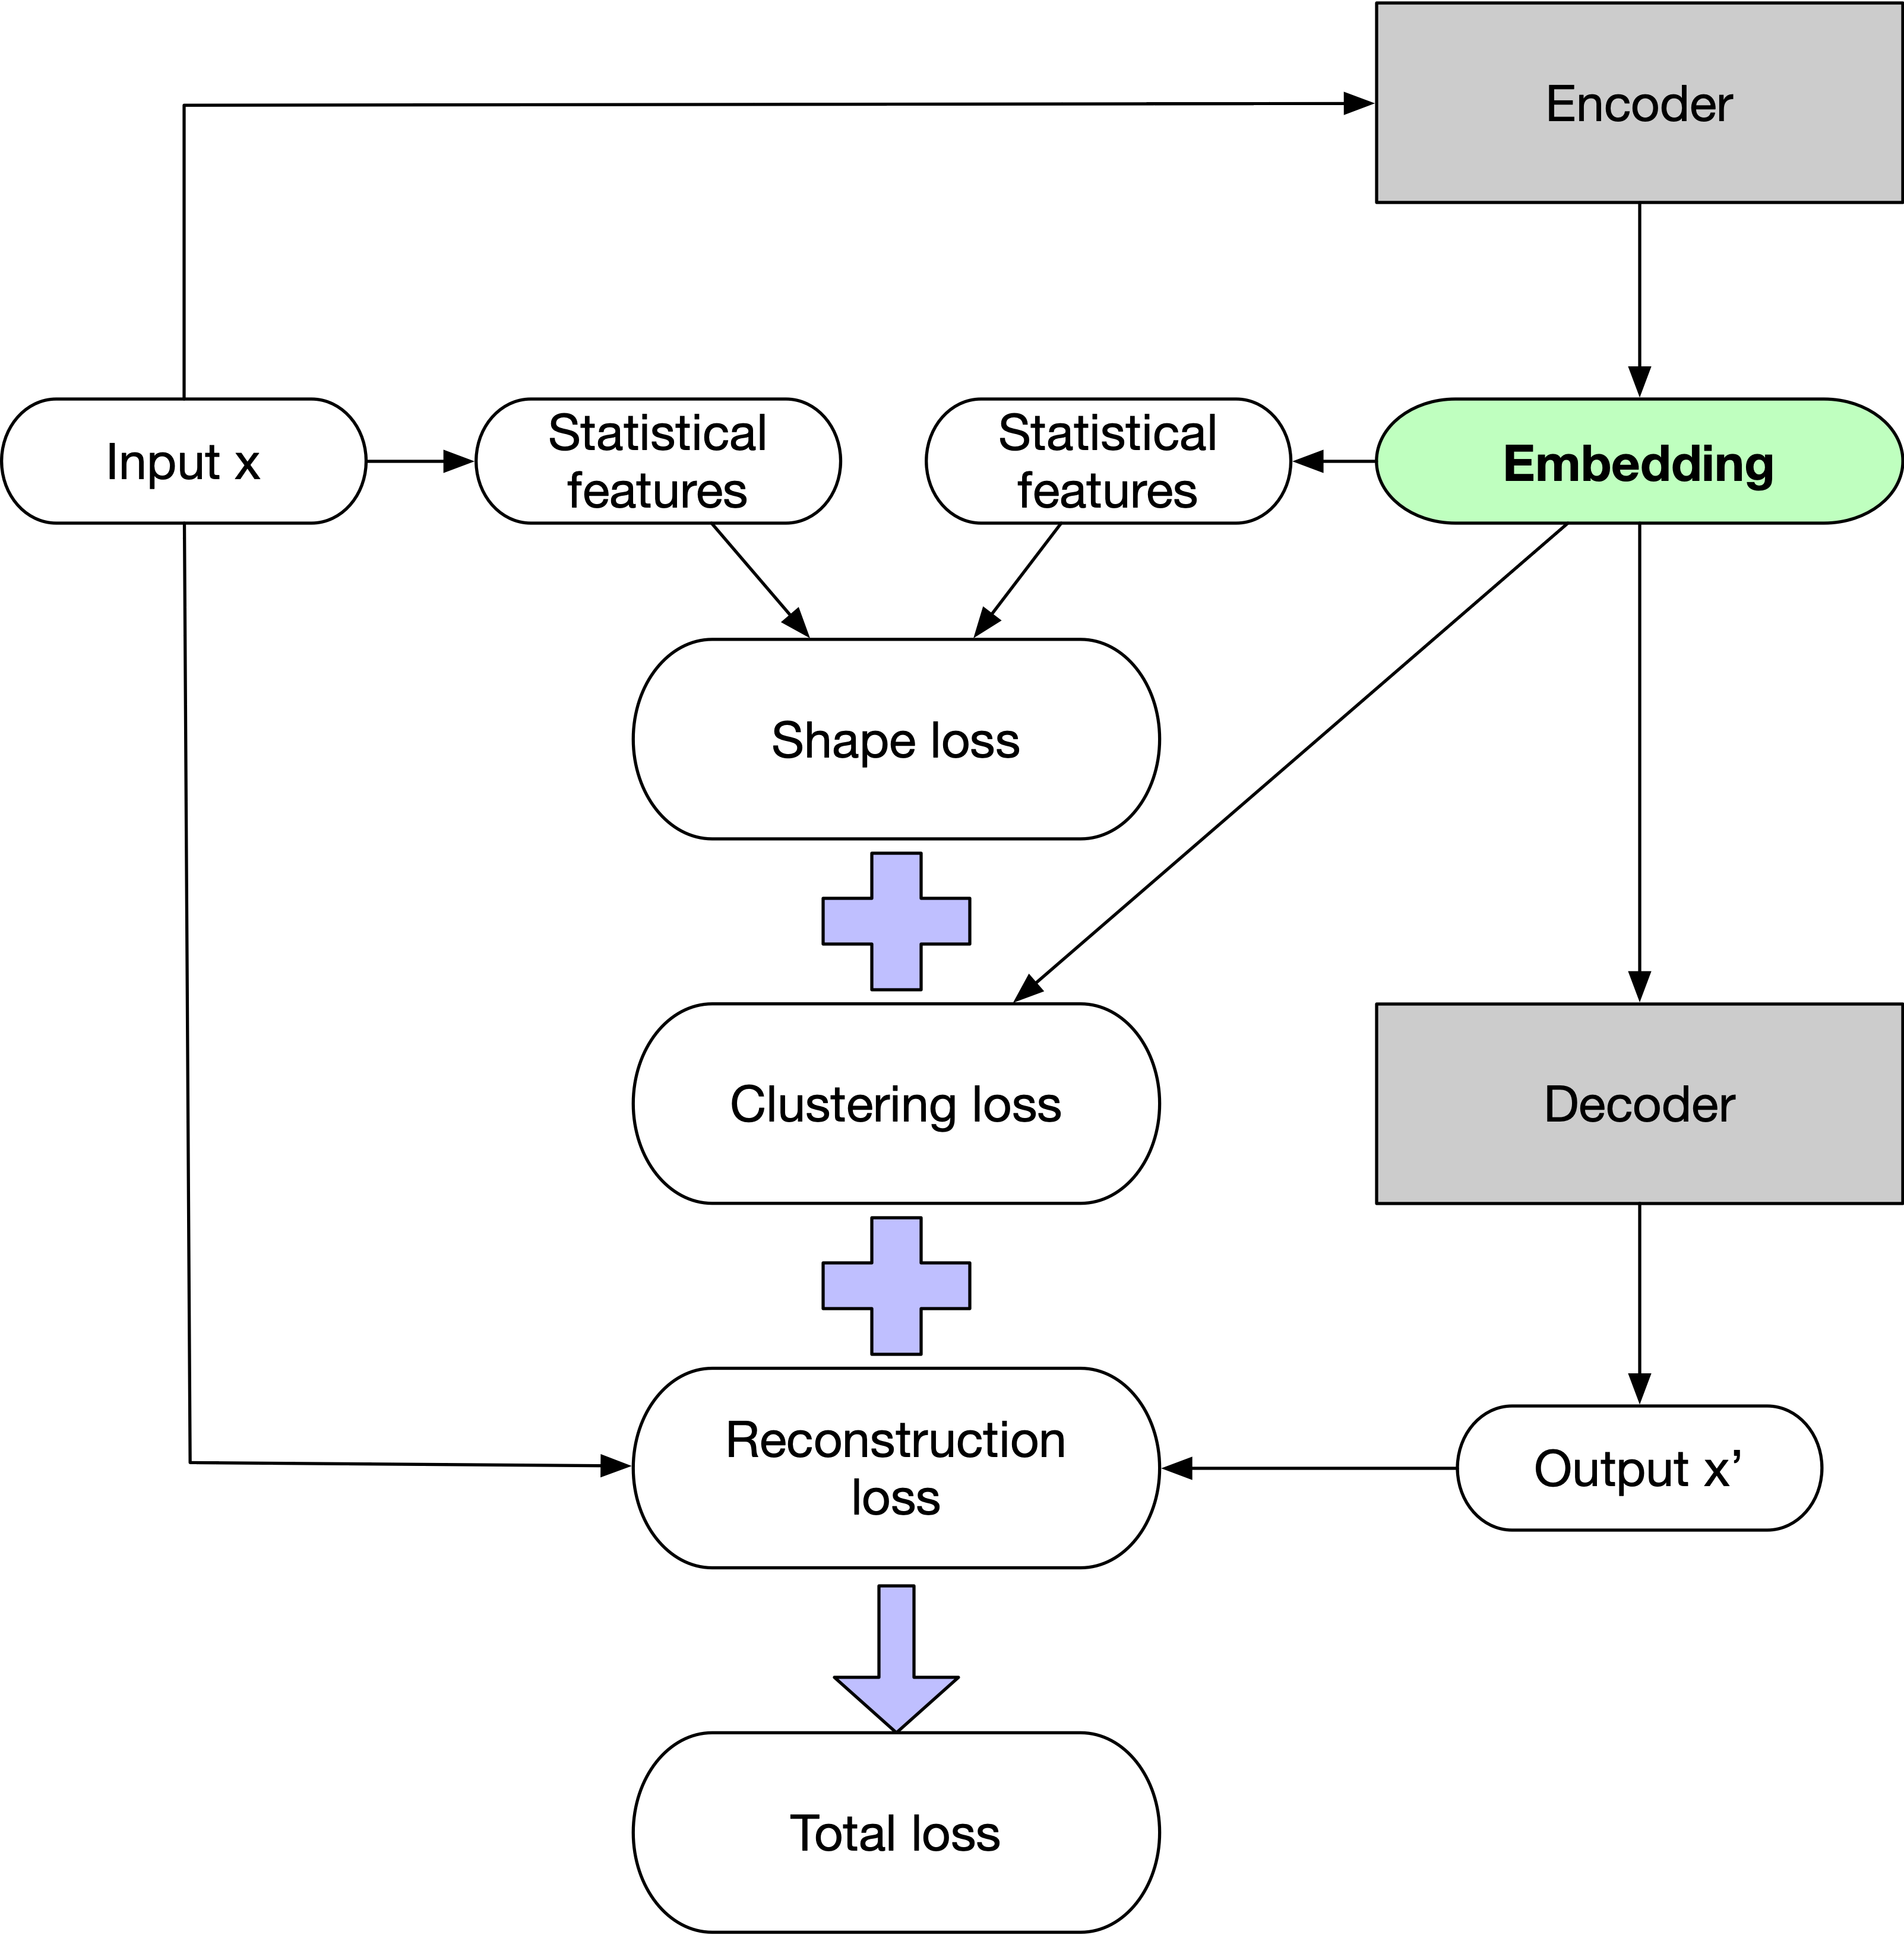
\includegraphics[width=0.6 \columnwidth]{sspcr1.png}
    \caption{General structure of SSPCR}
    \label{fig:sspcr1}
\end{figure}
\\Figure~\ref{fig:sspcr1} illustrates the how SSPCR works. SSPCR adpots the basic structure of the traditional autoencoders, expect that there are two more constraints: the shape loss and the clustering loss. In the training process, given a batch input vectors $X$, SSPCR will first extract their statistical features $S_X$, and then fed the raw sequences into the encoder. Then the encoder will map the original input sequences into a new feature space to get the new representations/embeddings of that data. The statistical feature set $S_E$ of the embeddings will be extracted and used to compute the shape loss. In the meanwhile, the clustering loss of that data batch $X$ will be computed with the Equation \ref{eq:kmeans2}. Follow the steps of common autoencoders, the embeddings will be fed into the decoder, where they will be used to reconstruct the original sequences. The reconstructed output $X'$ combined with the original sequences $X$ will then be used to compute the reconstruction loss based on the Equation \ref{eq:kmeans3}. Finally, those three loss will be summed together as the objective function for the training process, the equation is defined as:
\begin{equation}
    \mathcal{L}_{SSPCR} = \alpha \mathcal{L}_{shape} + \beta \mathcal{L}_{reconstruction} + \gamma  \mathcal{L}_{clustering}
    \label{eq:objective}
\end{equation}
Where $\alpha$, $\beta$ and $\gamma$ are the weights assigned to each loss. To be specific, $\mathcal{L}_{shape}$ encourages the encoder to produce embeddings encoded with most shape information of the input data, $\mathcal{L}_{reconstruction}$ forces the embeddings to preserve the most intrinsic properties of the input and makes them reconstructable, $\mathcal{L}_{clustering}$ encourages the embeddings to be distinguishable for clustering. It's worth mentioning that in the equation of $\mathcal{L}_{clustering}$, the cluster indicator matrix $F$ can be computed only when the data matrix $X$ is fixed, however, in SSPCR, $X$ is the embedding matrix that are learned. To make the reformulation applicable, SSPCR adpots Expectation Maximization (EM) approach to update the weights. Here the E step is fixing the $F$ and updating the $X$, and the M step is fixing the $X$ and updating the $F$, at the begining, $F$ is randomly initialized as an orthogonal matrix. Note that the updating of $F$ does not require backpropagation, it can be directly computed by SVD decomposition. In addition, $F$ should not be update at each training epoch, since that will make the training unstable. In terms of the shape loss, SSPCR also adpot the mean squared error to represent it. 
\\\\Currently, the statistical features selected are the same with those used in \cite{nanopoulos2001feature}: the mean value, standard deviation, skewness and kurtosis, their equations can be found in Section~\ref{sec:statistical}. Let $E$ denotes the embeddings, the shape loss computed with statistical features is defined as:
\begin{equation}
    \begin{aligned}
        \mathcal{L}_{shape\_statistical}(X,E) = \frac{1}{2|X|} \sum_{i=1}^{|X|} &  \left\| \mu(x_i) - \mu(e_i) \right\| ^2 + \left\| + \sigma(x_i) - \sigma(e_i) \right\| ^2 \\ 
        & + \left\| SKEW(x_i) - SKEW(e_i) \right\| ^2 \\
        & + \left\| KURT(x_i) - KURT(e_i) \right\| ^2
    \end{aligned}
    \label{eq:shapeloss1}
\end{equation}
The choice of statistical shape features are nontrivial and need human participation. The feature set selected here is preliminary, more features will be tested in the future work. To exclude the huamn participation, make the algorithm have less hyperparameters, another shape loss is proposed. This shape loss is inspired by the shape-preserved representations -- one can control the dimension of the input data by compression algorithms. This gives a hint that \textbf{the representation can be forced to approximate the compressed vector}. Let $\hat{X}$ denotes the compressed sequences, the compression-based shape loss is similar to the reconstruction loss, defined as:
\begin{equation}
    \mathcal{L}_{shape\_compression}(\hat{X},E) = \frac{1}{2|\hat{X}|}\sum_{i=1}^{|X|} \left\|\hat{x}_i - e_i \right\|^2
    \label{eq:shapeloss2}
\end{equation}
Downsampling is selected as the compression method since it produces the best results in the experiment. According to experimental results, the second shape loss produces slightly better partitions than the first one, but it has an obvious limitation that the dimension of the representation can not be greater than the original sequence.
\\\\Given the raw dataset $D$, the expected number of clusters $K$, the maximal training epochs, and the updating interval of $F$ $T$, the pseudocode of the SSPCR learning paradigm can be seen in Algorithm \ref{alg:sspcr}.
\begin{algorithm}[!htbp]
    \caption{SSPCR training method}
    \label{alg:sspcr}
    \LinesNumbered 
    \KwIn{$D$: Dataset $D=\{d_1,d_2\dots d_n\}$\newline
    $K$: number of clusters \newline
    $Epoch$: the number of maximum iterations \newline
    $T$: the time interval of updating the cluster indicator matrix $F$
    }
    \KwOut{$E$: the learned embeddings of $D$
    }
    Pre-process D \\
    Initialise an arbitrary orthogonal matrix $F$\\
    \For{$i = 1$ to $Epoch$}
    {
        \For{
            $X \in D_{batches}$
        }{
            Compute $E = encoder(X)$ \\
            Compute $\mathcal{L}_{shape}$ based on Equation \ref{eq:shapeloss1} or  \ref{eq:shapeloss2}\\
            Compute $\mathcal{L}_{clustering}(E)$ based on Equation \ref{eq:kmeans2}\\
            Compute $X' = decoder(E)$ \\
            Compute $\mathcal{L}_{reconstruction}(X,X')$ based on Equation \ref{eq:reconstruction} \\
            Compute the total loss $\mathcal{L}_{SSPCR}$ \\
            Update parameters $\theta$ of the neural network and the embeddings $E$ by back propagation \\
            \If{$i \% T = 0$}{
                SVD decomposite $E$ \\
                Update $F$ by composing the first $K$ singular vectors
            }
            \If{$early\_stop(\mathcal{L}_{SSPCR})$}{
                Stop iteration
            }
            
        }
    }
\end{algorithm}
\\\\The core part of SSPCR is the objective function, and there is no special requirement of the structure of the encoder and decoder. \textbf{For better comparison, the encoder of Time-series Transformer \cite{zerveas2020transformer} is chosen as the encoder of SSPCR in this project, while the decoder is a simple fully-connected layer}. The general model structure of Time-series Transformer is similar with the original Transformer (see Figure~\ref{fig:transformer}), expect the decoder is replaced by other customized neural networks. More detailed description of the original Transformer model can be found in \cite{vaswani2017attention}.
\begin{figure}[!htbp]
    \centering
    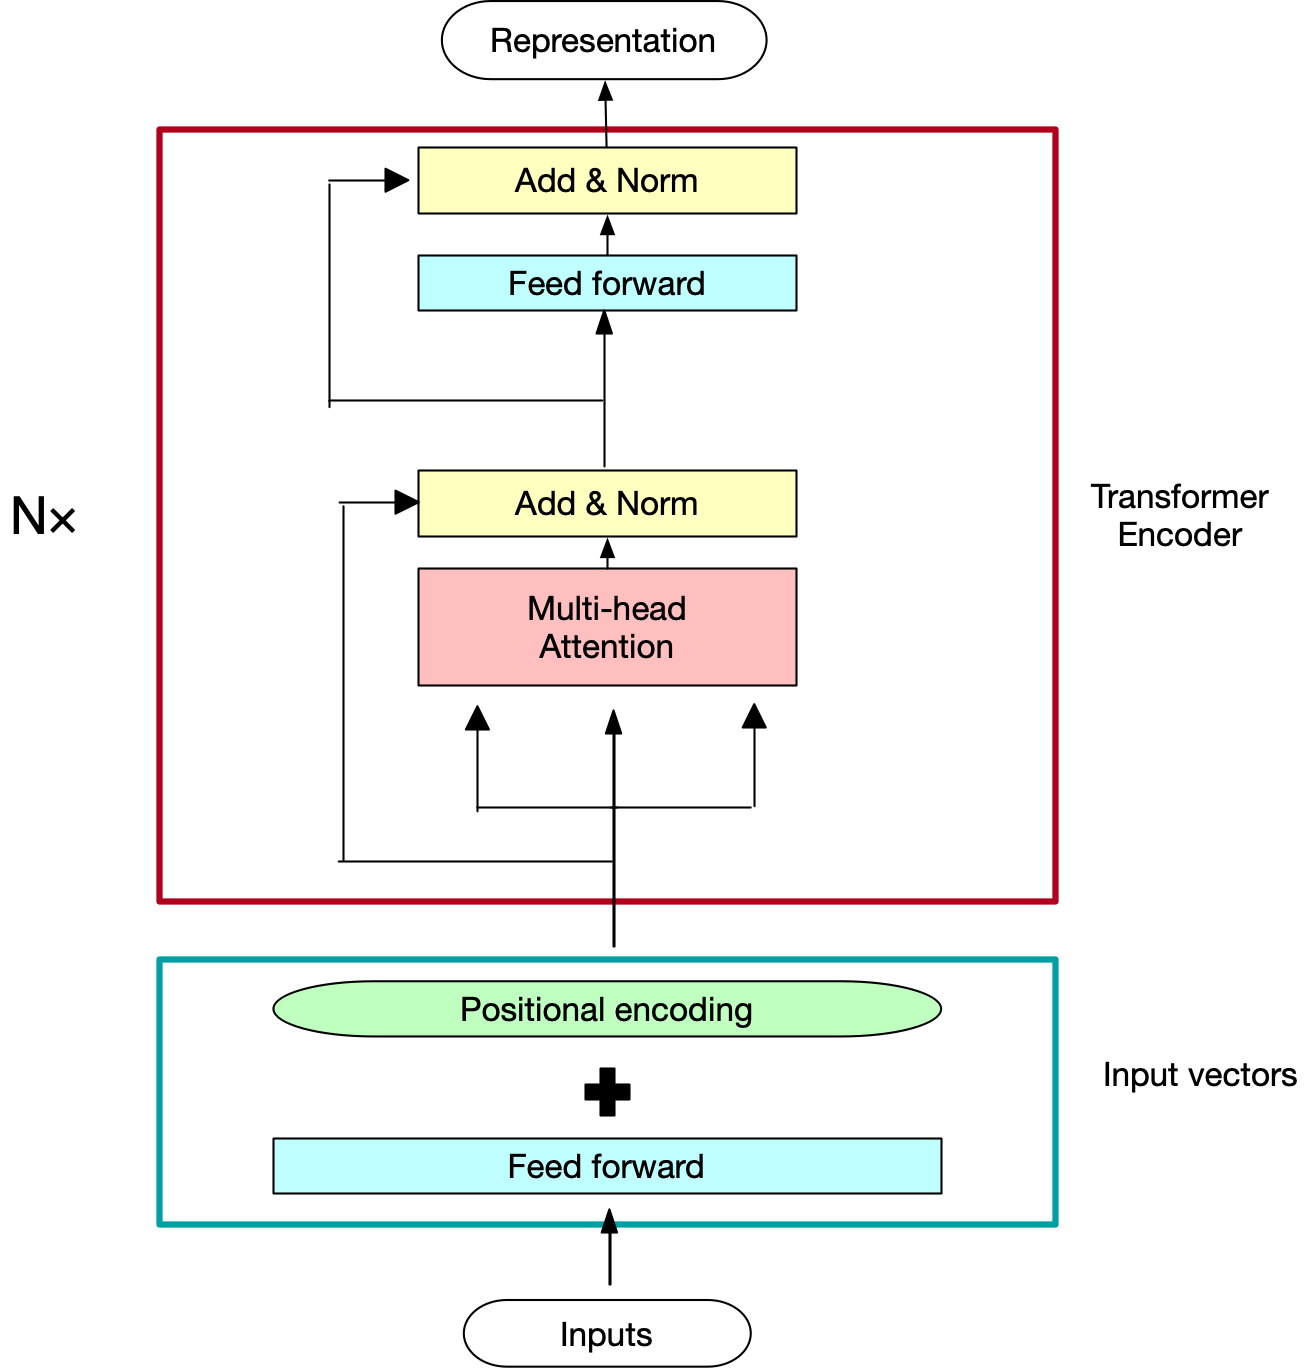
\includegraphics[width=0.5 \columnwidth]{transfomer.png}
    \caption{The structure of Transformer's encoder}
    \label{fig:transformer}
\end{figure}
\\\\Given a pre-processed data sample $X$ of length $w$ and $m$ variables ($m$ could be 1), Time-series Transformer first projects the data onto a $d$-dimensional feature space, where $d$ is a pre-defined dimension of the sequence representation in the model. Usually, such projection is done by a fully-connected layer. Since the model is a simple feed-forward neural network, it can overlook the ordering of input, which is quite important for time-series data such as stock sequences. To preserve the ordering information, a positional encoding $PE$ is added to the projected data $U$ before being fed into the encoder. Note that the positional encodings used in the Time-series Transformer is not the deterministic, sinusoidal encodings proposed in the original Transformer, instead, they are learnable weights. The encoder is formed by $N$ self-attention blocks, where each block takes the output from previous layer, transforms them into the query, key and value pairs. Then those pairs are used to compute the attention scores of the input. Residual and normalization layers are added to avoid vanishing gradients problem, guaranteeing the success of training. One different setting of the encoder is that it uses batch normalization rather than layer normalization, since the time-series sequence could have outliers that can rarely be found in natural language data. To handle with the problem that time-series sequences may have considerable variation in length, shorter sequences are padded with arbitrary values while longer sequences are truncated. To force the model to ignore the padded positions, an additional padding mask with large negative values on the padded positions are added to the attention scores before feeding them to the softmax layer of self-attention blocks. Figure~\ref{fig:irixpaysspcr} shows an example of applying SSPCR with Time-series Transformer to stock records of ``IRIX'' and ``Pay'' in 2011.
\begin{figure}[!htbp]
    \centering 
    \subfigure[Original sequences] { \label{fig:irixpay1} 
    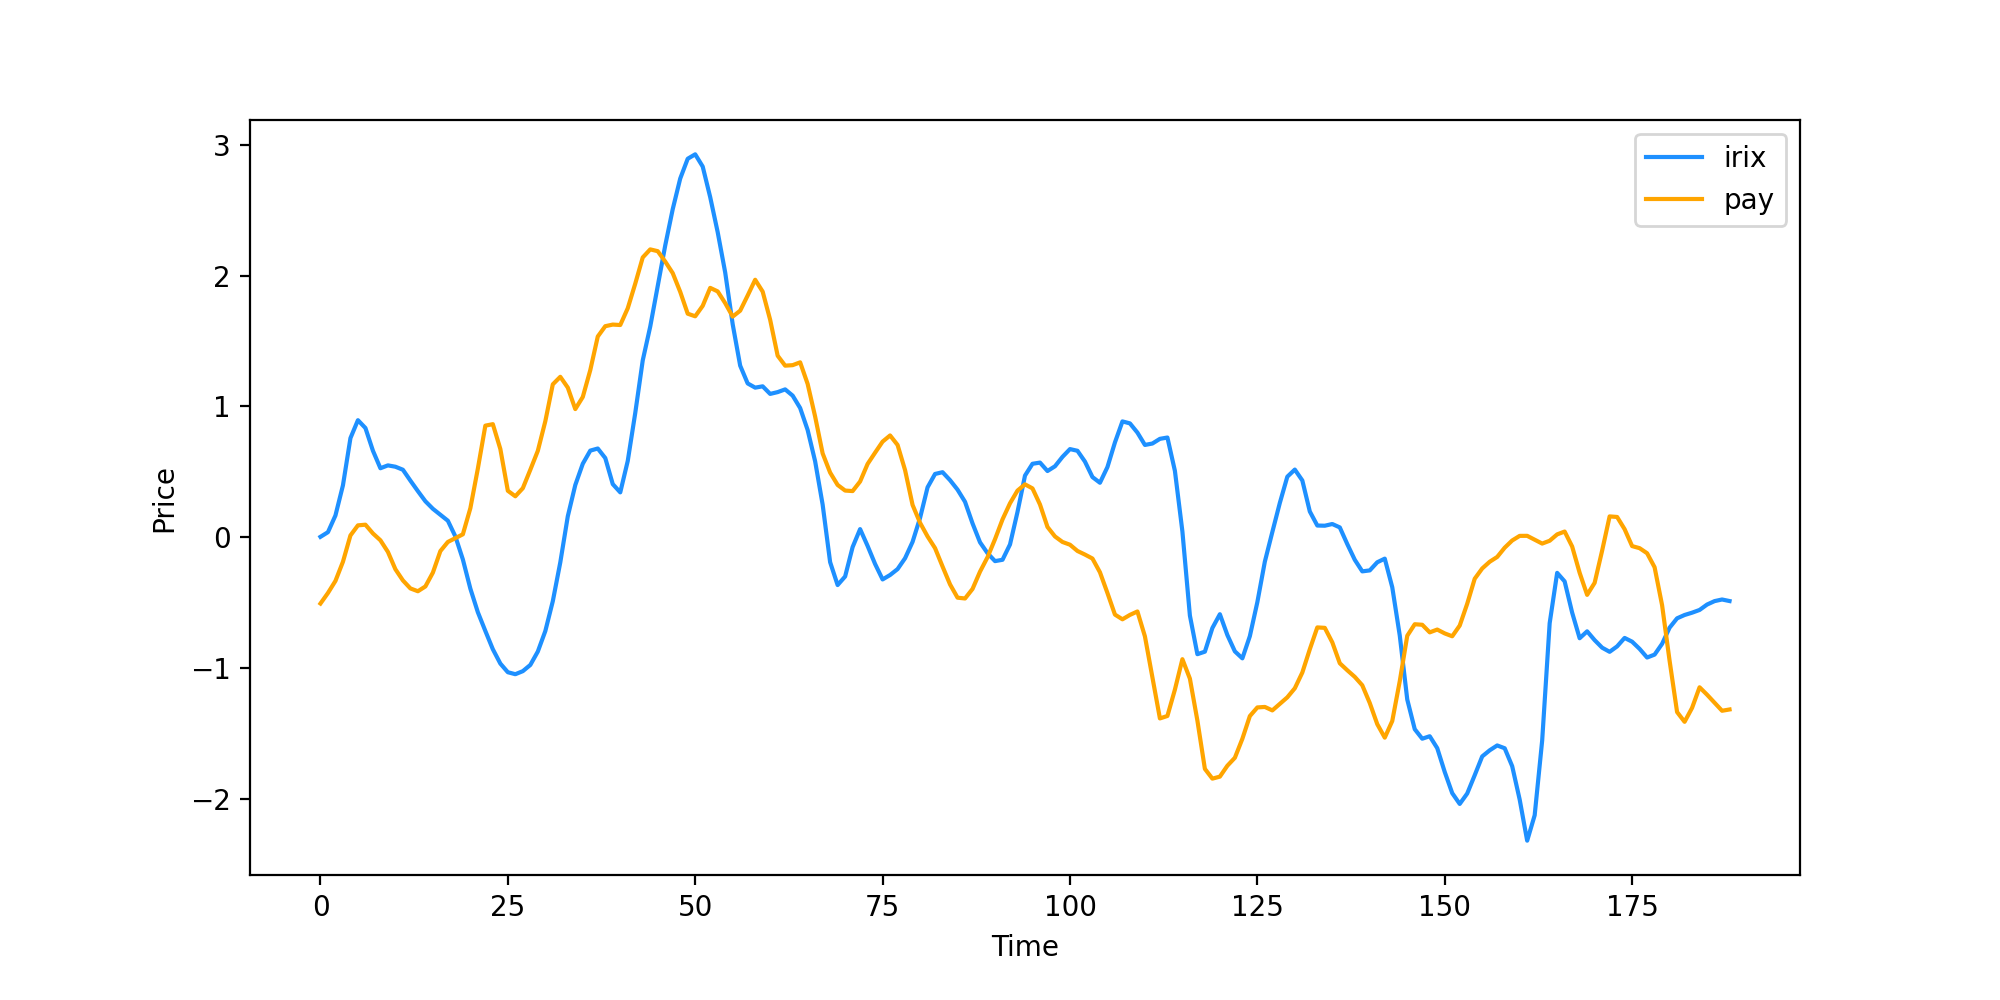
\includegraphics[width=0.4\columnwidth]{irixpay1.png} 
    } 
    \subfigure[SSPCR transformation] { \label{fig:irixpay2} 
    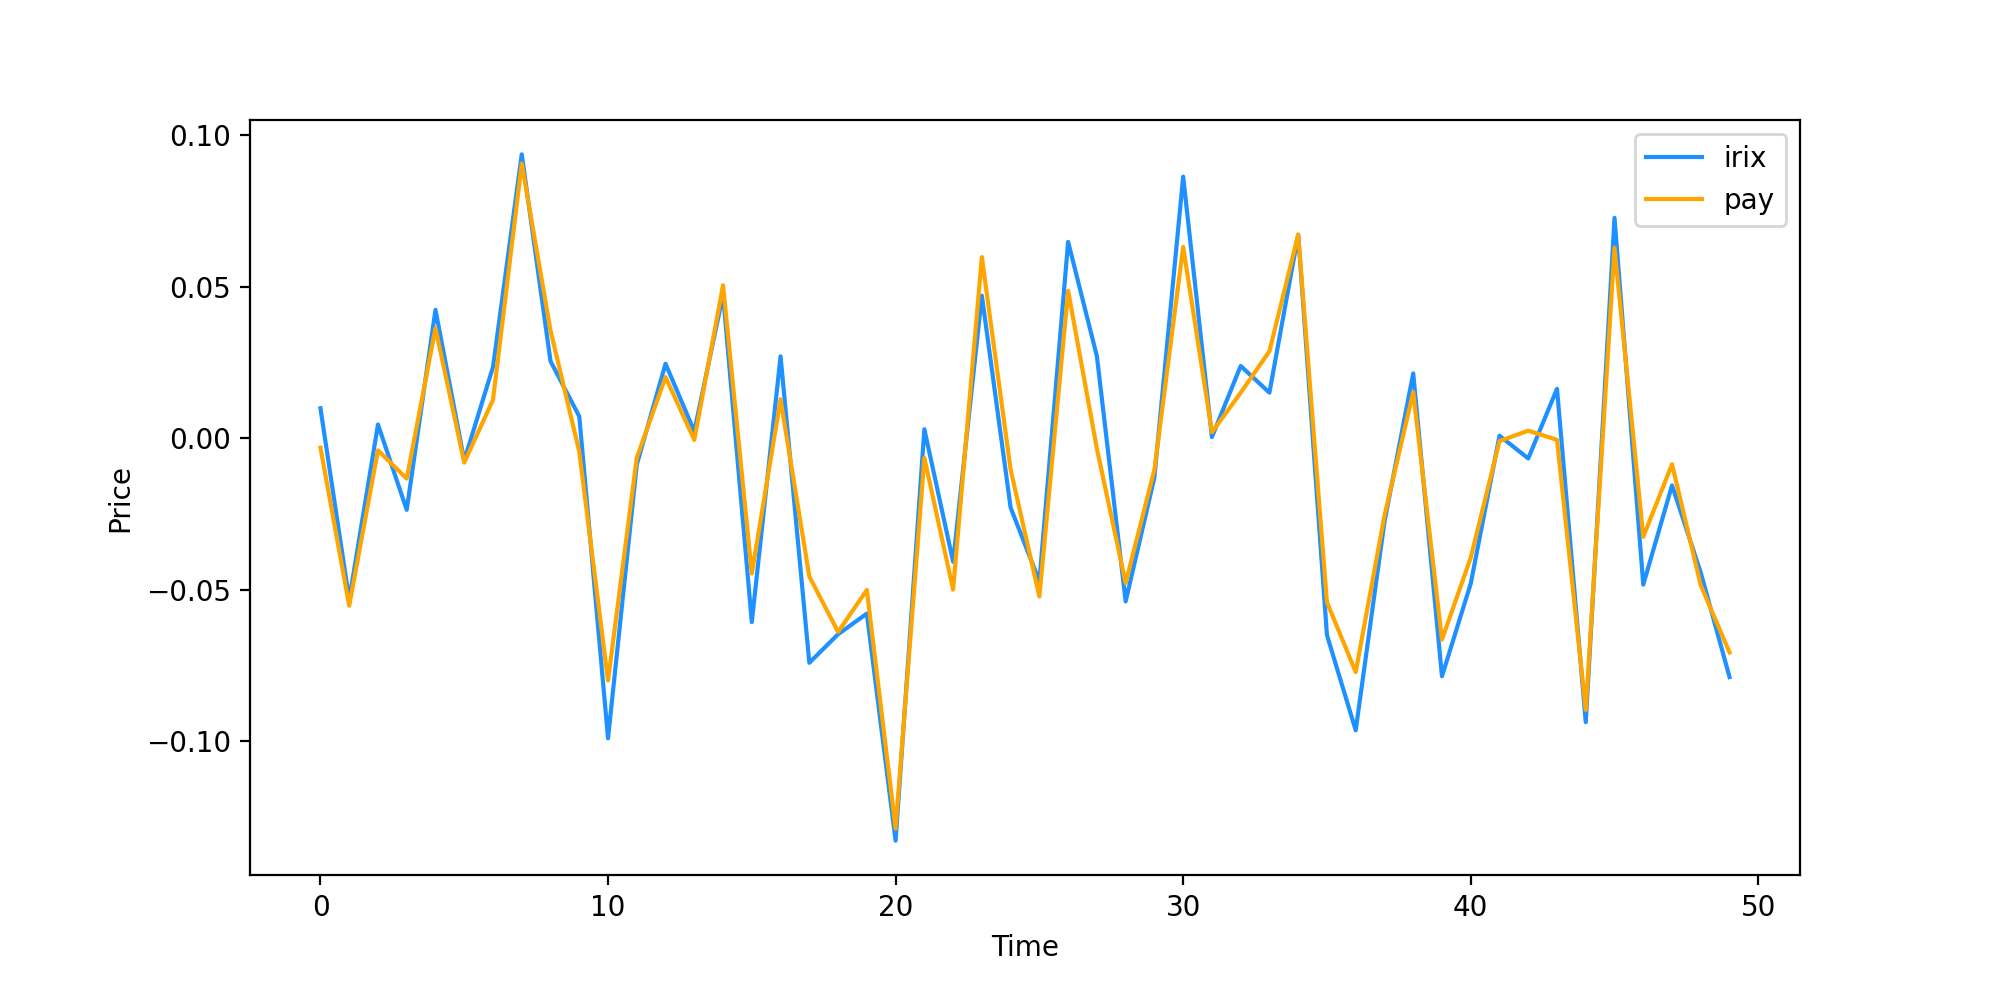
\includegraphics[width=0.4\columnwidth]{irixpay2.png} 
    } 
    \caption{ Example of SSPCR representation } 
    \label{fig:irixpaysspcr} 
\end{figure} 

\section{Chapter Summary}
This chapter introduces a novel representation learning algorithm designed for shape/trend-based time-series clustering tasks named as Semi-Shape-Preserved Clustering Representation (SSPCR), its pseudocode and the structure of the autoencoder used in the project. SSPCR are designed to take the advantages of both Shape-Preserved and Shape-Changed representations and discard their disadvantages. Semi-Shape-Preserved representations are expected to contain the most useful shape information while can unveil the intrinsic properties of the original data. Since the new vectors usually have different length, one can not force the representations to directly approximate the raw data. To solve this problem, two approaches are proposed: (1) using statistical features to represent the shape information, which doesn't refer to the length of sequences; (2) compressing the raw data to let them approximatable. These two approaches lead to two different shape loss functions. To make the representation suitable for clustering tasks, the objective function of traditional clustering algorithms within-cluster-scatter is added to the loss function. Due to the reformulation of within-cluster-scatter, its computation can be done by simple matrix production, and hence it can be optimized by gradient descent. The autoencoder used to test the effectiveness of SSPCR is the Time-series Transformer, but other autoencoders are also applicable. 